\documentclass{report}
\usepackage{lipsum} % for dummy text
\usepackage{draculatheme}
\usepackage{graphicx}
\usepackage{caption}
\usepackage{subfigure}
\usepackage{tabularx}
\usepackage{multirow}
\usepackage{amsmath}
\setcounter{secnumdepth}{0}

\title{Cubo - Memo}
\author{Botond Kovács, Frank Dierolf}

\begin{document}
\maketitle

\section{Introduction}

This document is a concise Buisness Plan.
It follows the 6 Page Memo Style, which got popular over Amazon's use in executive mettings.
I chose this structure because it inherits reading flow, aims executives and I feel comfortable with it.

First, let me introduce you to Cubo.
Cubo is a wooden cube, that you can place on every desk, coworking space, household and a great crafted piece of wood for every interior.
Cubo is also a Blockexplorer which adapts to the Users needs.
Cubo is the answer of Complexity and rooden language in the technology and especially the crypto space.
Cubo is a product of the Polkar - Team.
The team is combine of Botond, a Software Architect by profession and Frank, me, a Buisness Developer.

Before we outline the core elements, lets go back in time and tell our Backstory.

\section{The Backstory}
Franks story starts 3 years ago.
Crypto was just on the rise.
Me, Frank, just started out in conquering this area.
The first thing that stood appart compare to anything else that i encountered is, the language.
Its scary, unpleasant and feels wanna be smart in many corners.

Nontheless after a brief of time, i got used to it and adopted it.
The obvious happend. Another Problem appeared.
Noone understood me and to communicate crypto ideas to non crypto people is an nightmare.
Thats not the first time that i encounter this issue.
f.e. the medical industry shares the same issue.

I did, what i usually do. I simplify. Get rid of the ideas, get rid of the concepts, get rid of the buzzwords.
Get as close to the already known as possible. That leads to a point where i acquired a language thats catchy and understandable.
Even for Grandma.

It has a drawback. Its worth taking but a drawback nontheless.
Its not appealing for Business and Technology enviorment. People smile over this kind of communciation style.
But the right language lies where the market sits. The market sits in the everydays.
Things that people  buy in a supermarket, that people buy in a drug store, that people buy in amazon, that people buy ...

If Crypto wants high adoption, then lets switch gears and bring our great tools in every shelf, let people explore it by themselve and make money meanwhile.

Now, to the current time.
Botond and Me met on another Coding Competion. It was just us two in a team.
We had great fun together.
Admiration of each other was there from the get go.
Everyone throw something on the table, which the other person saw extrem rarely before.

We decided to go for another round, choose Dora Hacks Polkadot Hack and throw a coin for which category we are tackling.
Category Polkadot ecological developer tools.

\newpage

\section{Cubo}

We need an Idea. Botond came up with a AI blockexplorer.
You type what you want to get what you asked for.
I thought about an AR Cube. Holograms are sized, colored, animated based on Blockchain Data.
Inspired by one the sucess stories in the Auguemted Reality space, called Merge Cube.
So met in the middle and come up with Cubo.

Then we casted our spells, one after the other. We scratched Software Design Sheet.
We 3D Printed first Prototype.
We attach QR Codes.
We scratched ai driven visualtion engine, inspired templating engines.
We decided for going with search for configuration of visualtions.
We decided to add Dashboard Utilizies.
We redesign the Cube, lasered it out, stiched it togehter.
We scratch around in Figma for good intiutive layout and userfriendly UX.
We made simple user tests and collect some feedback.
We decided on a useful repo structure.
We added docs, presenation, buisnessplan, pitch deck to round it up.
2 weeks are gone, deadline is there and we are happy. Top notch timing for upcomming christmas.

\begin{figure}[hbp]
	\centering
	\subfigure[Configuarable Dashboard]{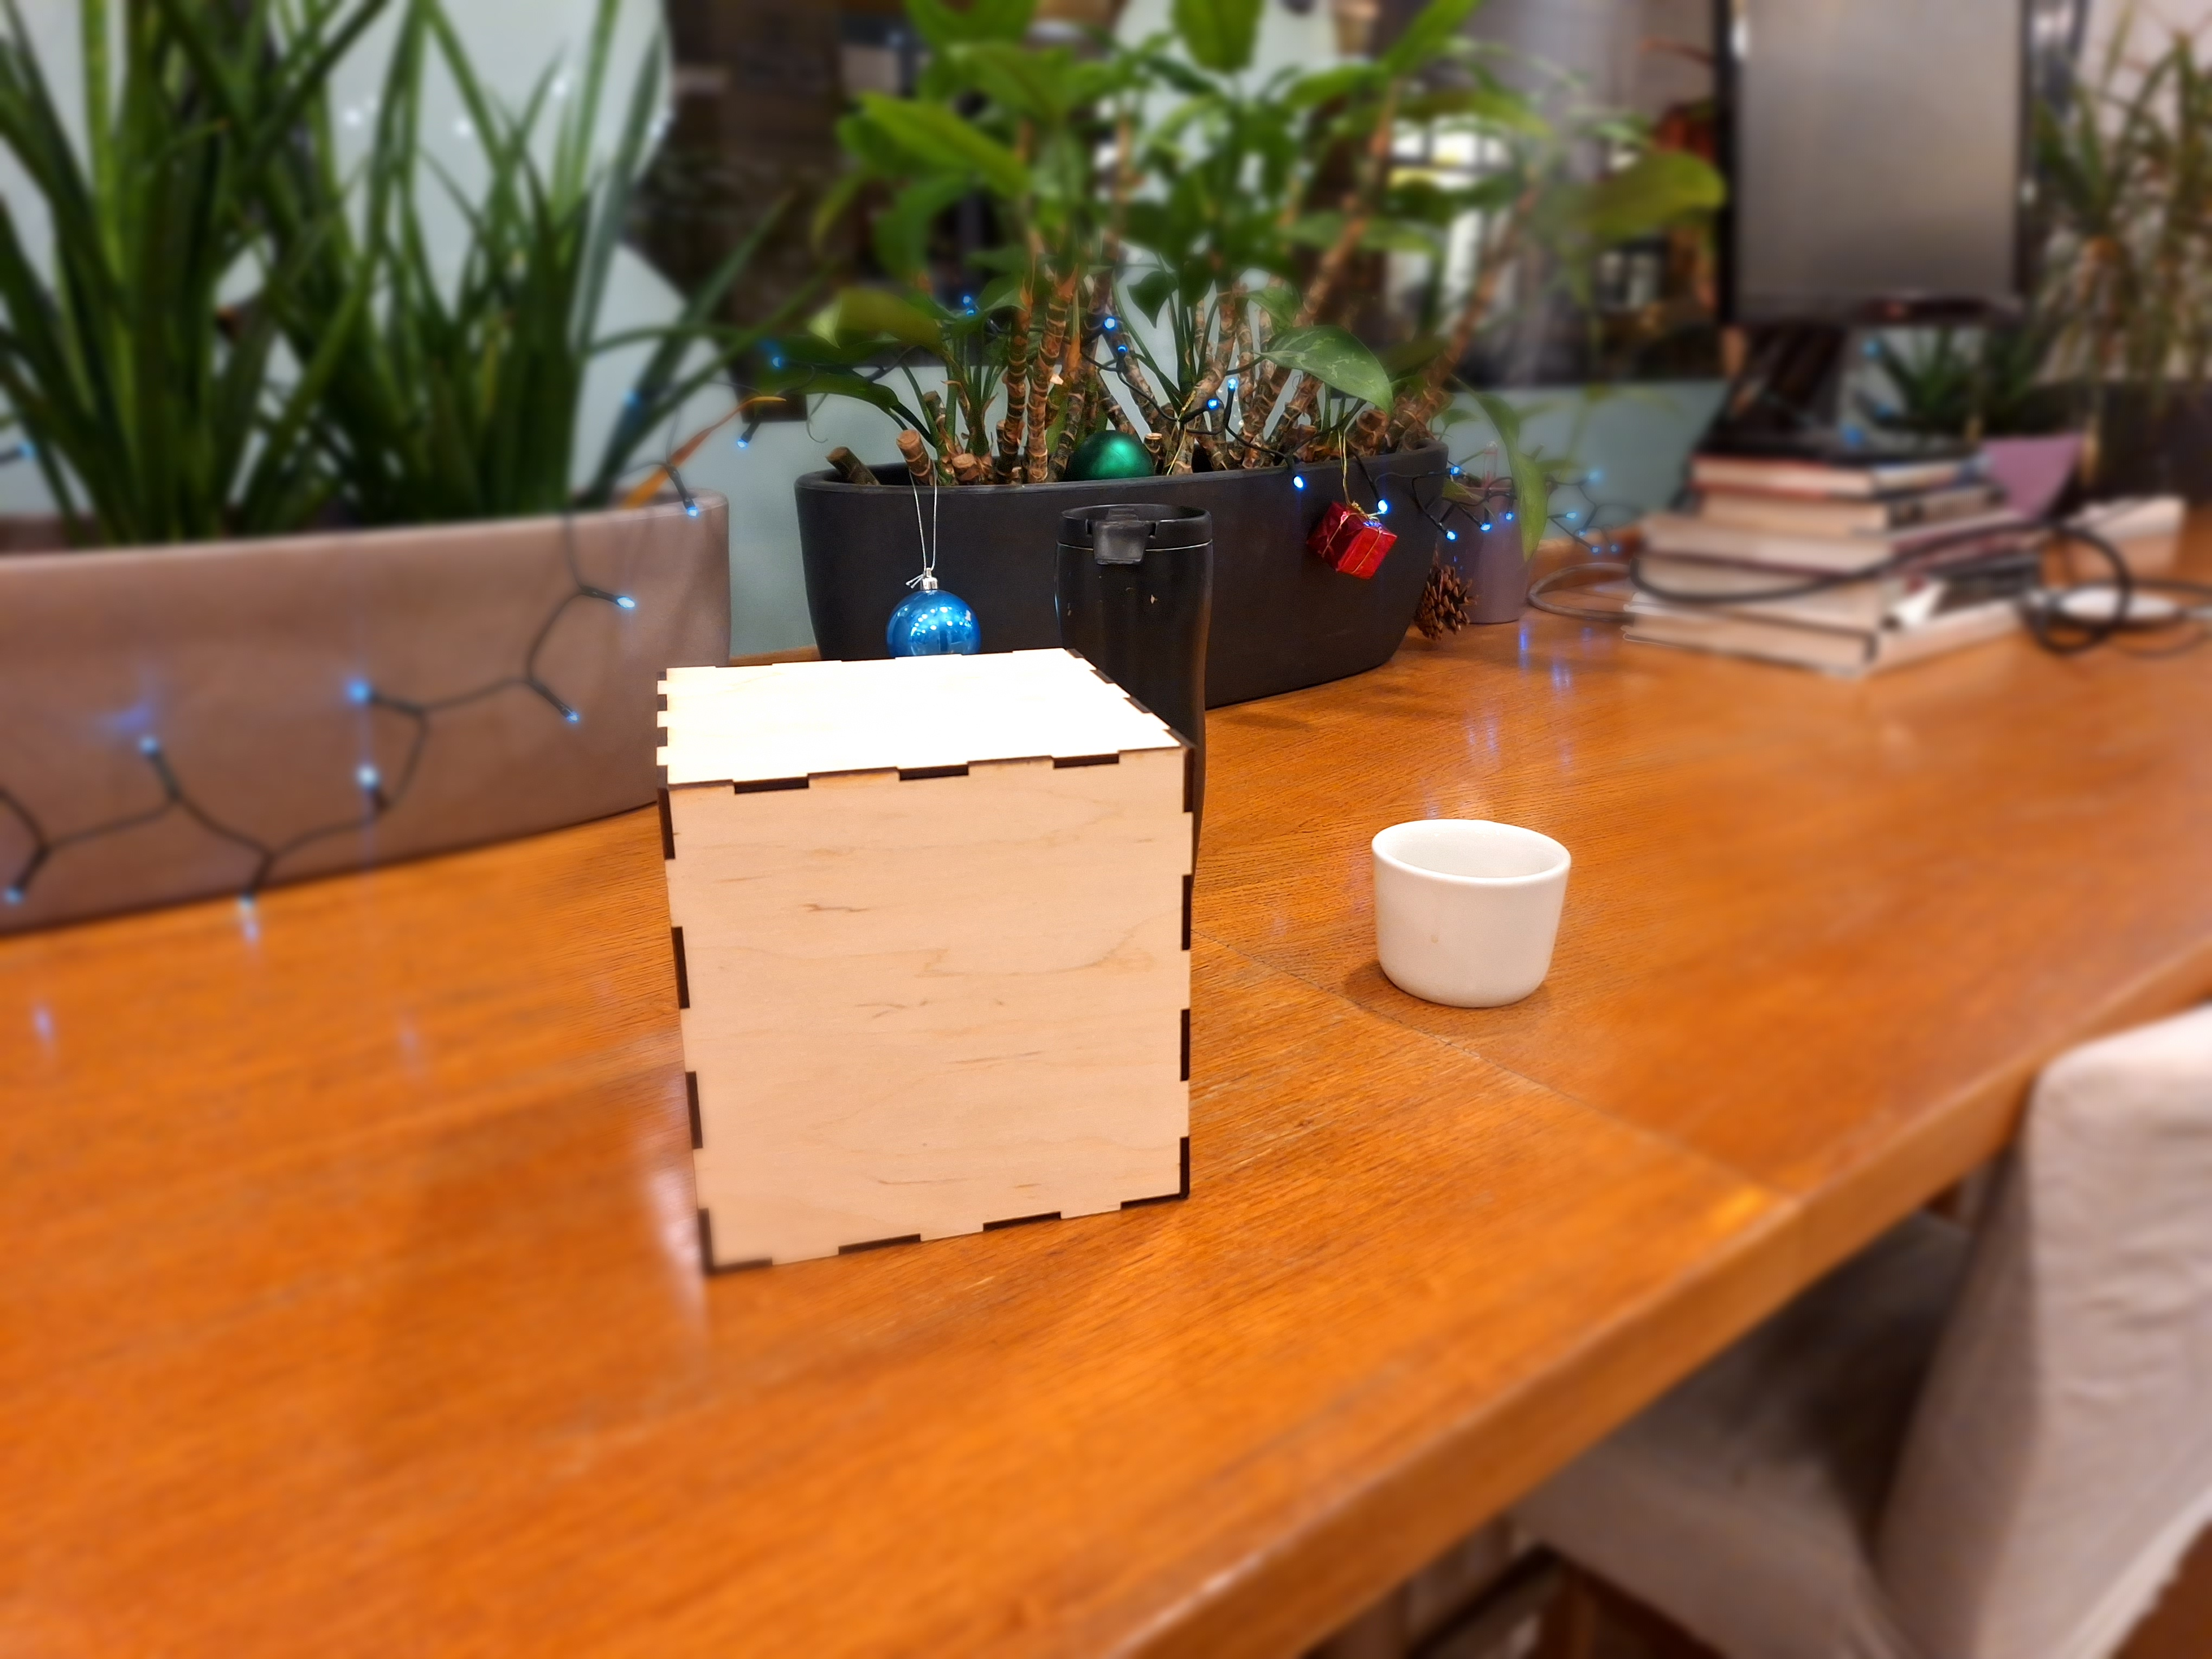
\includegraphics[width=0.4\textwidth]{./Cubo.jpg}}
	\hspace{1cm}
	\subfigure[Physical Product]{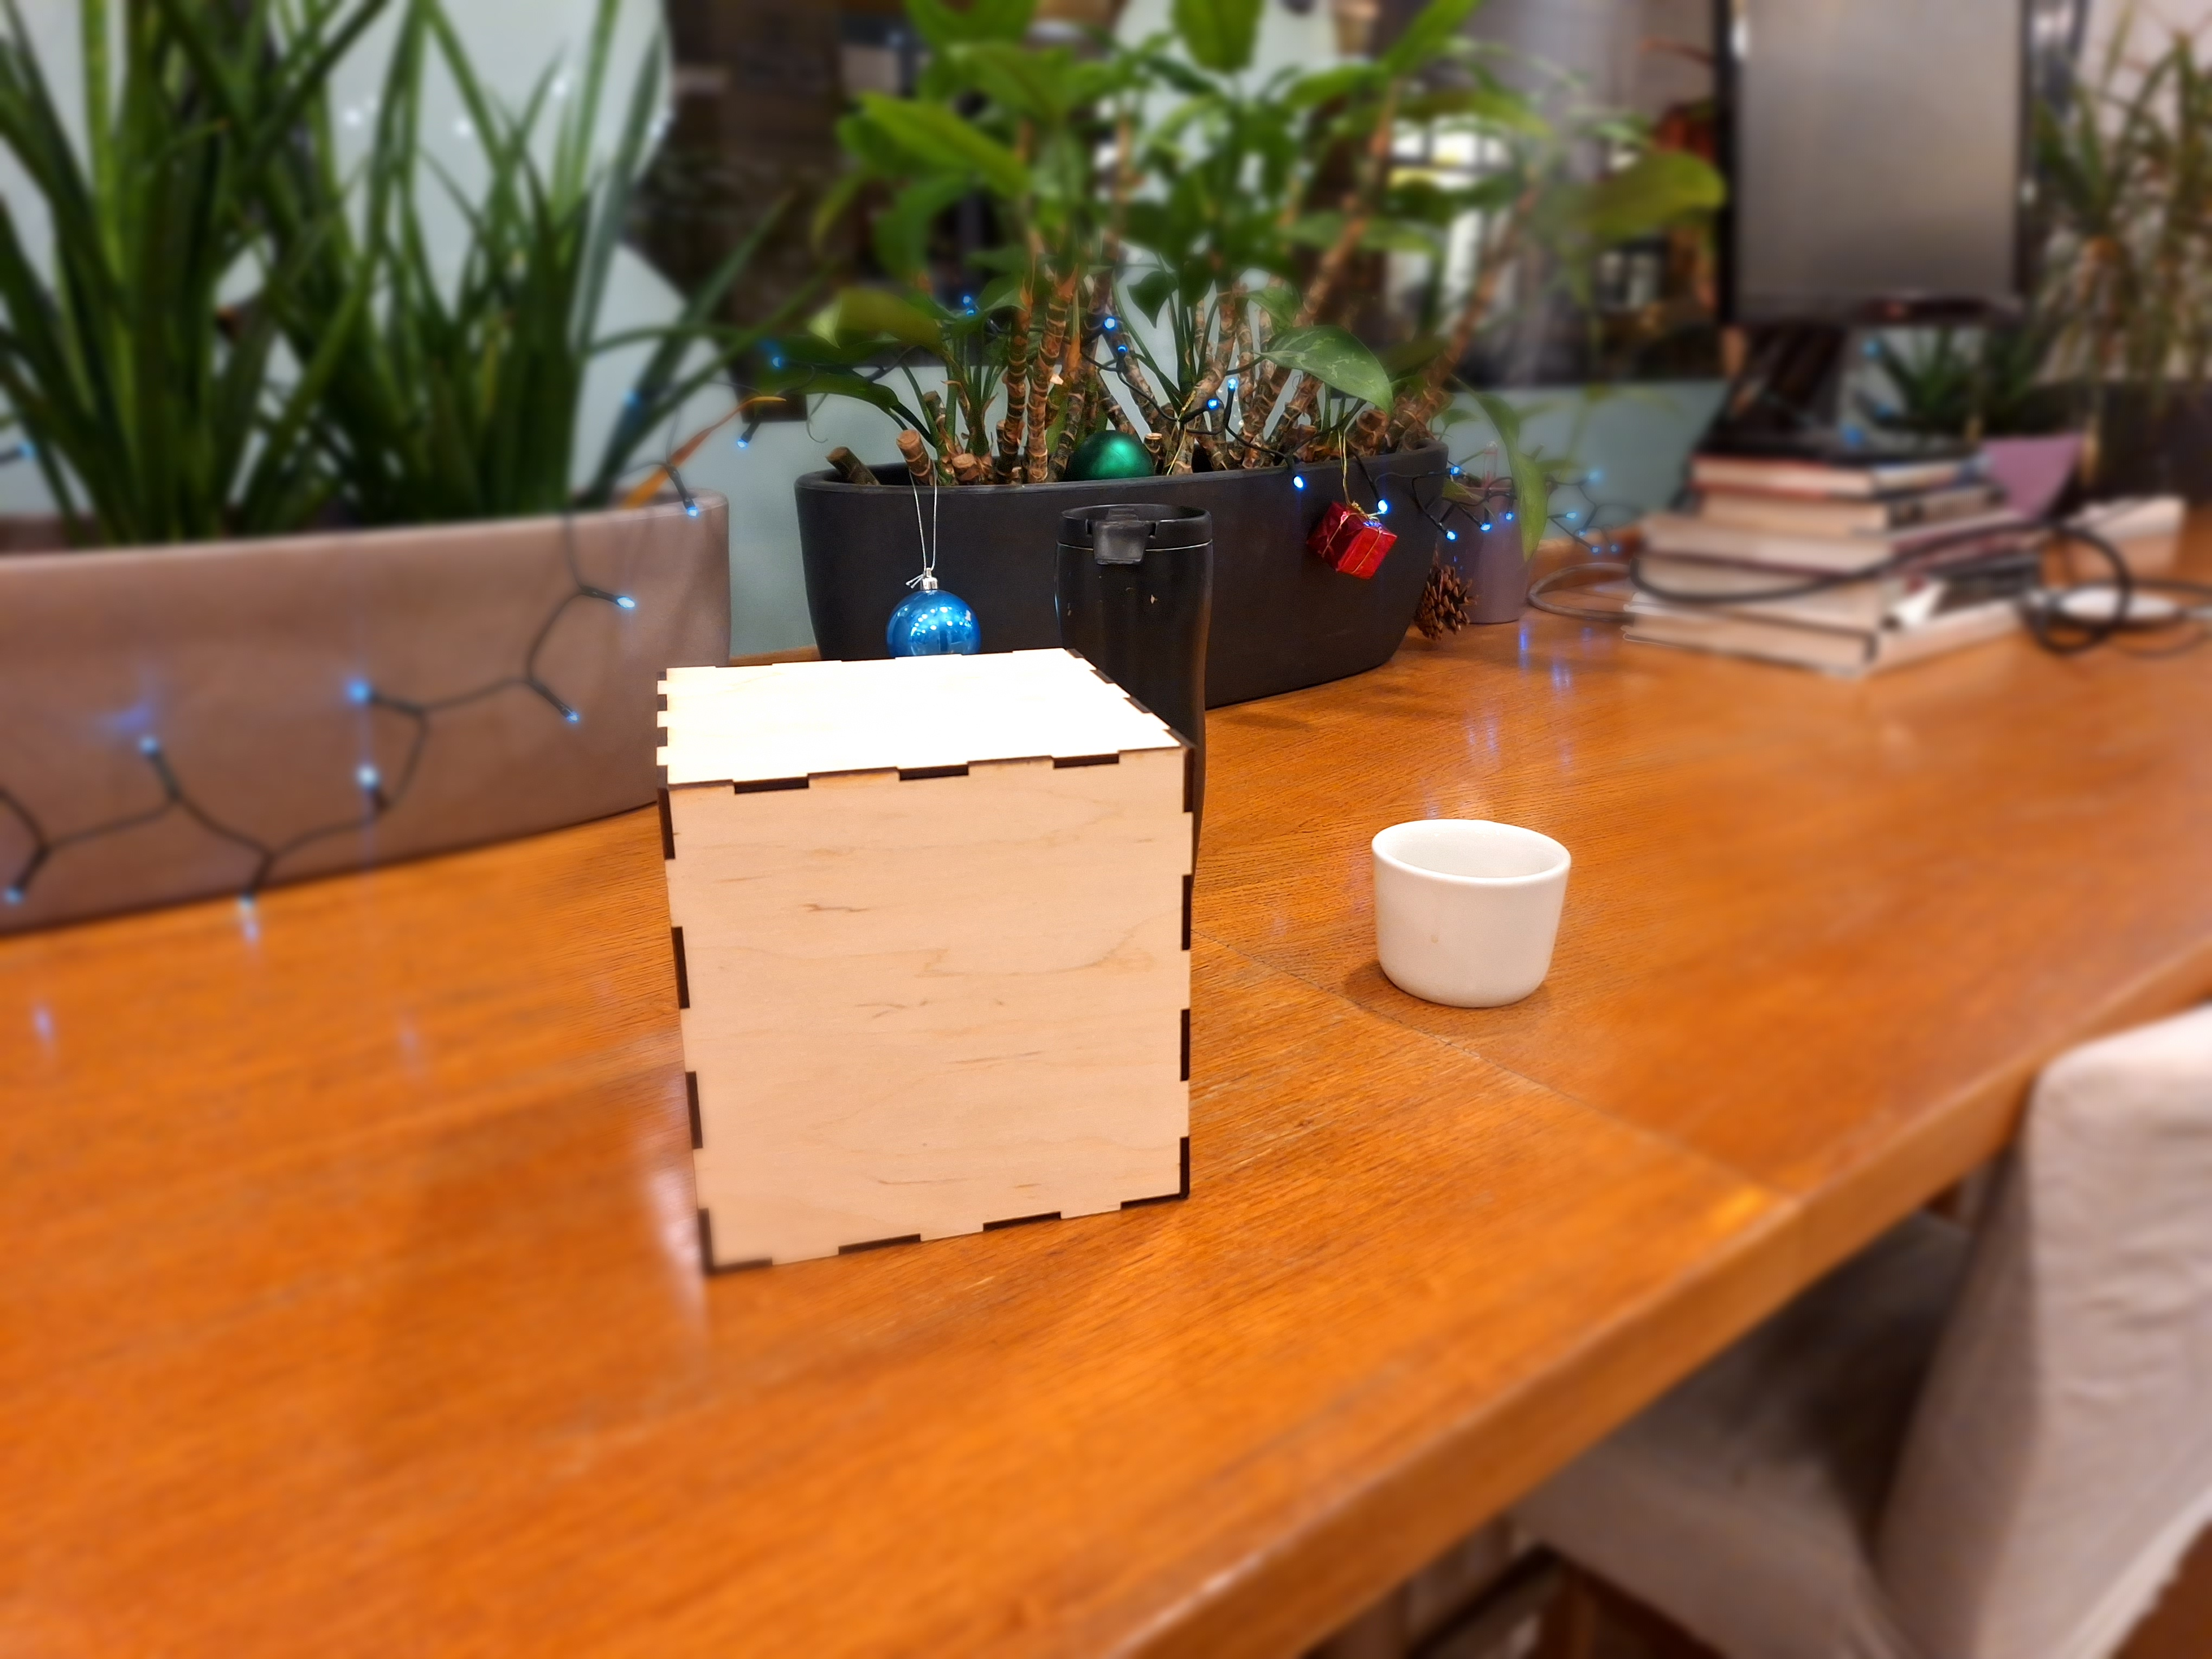
\includegraphics[width=0.4\textwidth]{./Cubo.jpg}}
	\caption{Cubo}
	\label{fig:Cubo}
\end{figure}

Back to buisness. How we plan to make money.
Like always, there are multiple tactics to approach a market.
I choose to structure the following section in Usersgroups.
Every Usergroup gets market approach.
Every buisness follows the following formula to reach sucess.

\begin{equation}
	\text{Earnings} = \text{Income} - \text{Cost}
\end{equation}

So every market approach has a table which displays earnings, income and cost per sell.

\begin{equation}
	\frac{\text{Earnings}}{\text{Sold}} = \frac{\text{Income} - \text{ProductionCost} - \text{TaxCost} - \text{HRCost}}{\text{Sold}}
\end{equation}

Cost will be only Production Cost per Sell.
Tax and Salaries are not included. The purpose is to get a comparision of earnings per sell.

\newpage

\section{Tactics}

\subsection{Usergroup A - Everyones: We sell Cubo's}

\begin{table}[hbp]
	\centering
	\captionsetup{justification=raggedright}
	\caption{Income over sold Products}
	\label{tab:sales}
	\begin{tabular}{|p{2cm}|p{2cm}|p{2cm}|p{2cm}|}
		\hline
		\textbf{Sold} & \textbf{Earnings} & \textbf{Income} & \textbf{Cost} \\
		\hline
		1             & \$40              & \$50            & \$10          \\
		\hline
		10            & \$400             & \$500           & \$100         \\
		\hline
		100           & \$4000            & \$5000          & \$1000        \\
		\hline
		1000          & \$40000           & \$50000         & \$10000       \\
		\hline
		10000         & \$400000          & \$500000        & \$100000      \\
		\hline
	\end{tabular}
\end{table}

Selling Cubos is the simplest approach.
It aims for the everyones.
Cubo gets seen as a nice piece of Furniture with Holograms.
Cubo seen as Blockexplorer is not important.

The Market approach is take the phone, call people and extend on it.
It does the thing.
Calling friends on the first day and ask if they wanna buy a cubo.
That leads the following: In the first day 10 leads, in a week 70 leads, in a month I have 240.
Scaling via social media and creating content to build a base.
Further scaling via offering other plattforms, ebay, etsy, amazon, ... .
Always collecting feedback and input.

Iterate and listen is underlying philosphy.

\newpage

\subsection{Usergroup B - Techies: We sell Access Tokens}
\begin{table}[htp]
	\centering
	\captionsetup{justification=raggedright}
	\caption{Income over sold Products}
	\begin{tabular}{|p{2cm}|p{2cm}|p{2cm}|p{2cm}|}
		\hline
		\textbf{Sold} & \textbf{Income} & \textbf{Earnings} & \textbf{Cost} \\
		\hline
		1             & \$-9            & \$1               & \$10          \\
		\hline
		10            & \$0             & \$10              & \$10          \\
		\hline
		100           & \$90            & \$100             & \$10          \\
		\hline
		1000          & \$990           & \$1000            & \$10          \\
		\hline
		10000         & \$9990          & \$10000           & \$10          \\
		\hline
	\end{tabular}
\end{table}

Selling Access Tokens is an lesser simpler approach.
It aims for the Techies.
Cubo gets not seen as a nice piece of Furniture with Holograms.
Cubo gets seen as Blockexplorer.

The Market approach is create dashboard which delivers good uptodate date data.
Create user test and listen extremly carefully to the Techies.
Identify their needs and implent one data set after another.
The semantic search feature for asking what the Techie wants and present them the fitting dashboard becomes absolute crucial.
Cubo has to reach a level where it competes with standard Blockexplorer.
After etablish a solid alternative, the token sells come. It has to be product focus market approach.

Focusing on delivering the most intuitive Blockexplorer is the underlying philosphy.

\newpage

\subsection{Usergroup X - X: We sell X}

In this section we just list a explored Concepts of how to apprach the market with Cubo.
We structured them in short and long term tactics and named the according Usergroups.

\subsubsection{Short Term}

\begin{table}[hbp]
	\centering
	\caption{Usergroup, Sell, Description}
	\label{tab:salesShort}
	\renewcommand{\arraystretch}{1.25}
	\begin{tabularx}{\textwidth}{p{3.5cm}|p{3cm}|p{4.5cm}}
		\hline
		\textbf{Usergroup}  & \textbf{Sell} & \textbf{Description}                                                          \\
		\hline
		\hline
		Everyones           & Cubo          & We well Cubos                                                                 \\
		\hline
		Interior Enthusiats & AR Furniture  & We sell AR Furniture                                                          \\
		\hline
		Degens              & Tokens        & We sell Tokens via ICO, Utlitiy Access token, Swap Tokens, Coupon Tokens, ... \\
		\hline
		Everyones           & Ads           & We sell indivual ads to everyone for crypto products                          \\
		\hline
	\end{tabularx}
\end{table}

\subsubsection{Long Term}

\begin{table}[hbp]
	\centering
	\caption{Usergroup, Sell, Description}
	\label{tab:salesLong}
	\renewcommand{\arraystretch}{1.25}
	\begin{tabularx}{\textwidth}{p{3.5cm}|p{3cm}|p{4.5cm}}
		\hline
		\textbf{Usergroup}    & \textbf{Sell}      & \textbf{Description}                                                    \\
		\hline
		\hline
		Product Companies     & AR Tools           & We sell AR Tools for Product Companies                                  \\
		\hline
		XR Companies          & Handhel Controller & We sell hanndheld controllers for XR Companies                          \\
		\hline
		Paperful Organisition & QR Code Tech       & We Sell qr code technology to replace paperfull organisation            \\
		\hline
		Crypto Companies      & Api                & We sell api usage for getting data like graphs and datasets             \\
		\hline
		Data Analysts         & Visualtion         & We sell visulation for data scientist                                   \\
		\hline
		Creators              & Plattform usage    & We sell plattform usage to creators of data visulation or data creation \\
		\hline
		Companies             & Bundles            & We sell bundles of datasets and visualisation packages                  \\
		\hline
	\end{tabularx}
\end{table}

\newpage

\section{Conclusion}

Thruh time constrains, we ask chat gpt to write a nice conclusion with the following bullet point, that we wanna get crossed.

\begin{quote}
	The inputed bullet points:
	\begin{itemize}
		\item Our product is Cubo.
		\item Cubo is wooden interior piece and a block explorer.
		\item Its unique selling point is its simplicity
		\item a. augmented reality visualizations based on blockchain data.
		\item b. user-friendly block explorer (ask and get)
		\item User tests are positive.
		\item We are satisfied with the progress.
	\end{itemize}
\end{quote}

\subsection{The GPT Concluions:}

In conclusion, Cubo is a unique and innovative product that aims to simplify the complexity of the crypto space. With its wooden cube design and dual functionality as a stylish interior decor piece and a block explorer, Cubo offers a visually appealing and user-friendly solution.

The key selling points of Cubo are its simplicity and user-friendly features. By removing the language barrier and providing intuitive search functionality, Cubo allows individuals, regardless of their technical background, to easily explore and understand blockchain data. The addition of augmented reality visualizations further enhances the user experience and makes complex concepts more accessible.

Although we have already conducted successful user tests and received positive feedback, we are continuously striving to improve and refine Cubo. We value user feedback and will continue to iterate on the product to ensure it meets the needs and expectations of our diverse user base.

In terms of market approach, we have developed tailored strategies to target different user groups effectively. By selling Cubo as a stylish piece of furniture to interior enthusiasts and offering access tokens to cater to the needs of the tech-savvy, we aim to maximize our market reach and drive widespread adoption of Cubo.

In conclusion, Cubo has the potential to revolutionize the way individuals interact with and understand blockchain technology. With its simplicity, visual appeal, and user-friendly features, Cubo is poised to make crypto more accessible and bring it into the everyday lives of people. We are confident in the success of Cubo and are dedicated to continuously improving and expanding the product to meet the evolving needs of our users.

\end{document}
